\documentclass[11pt,a4paper]{article}

\usepackage[utf8]{inputenc}
\usepackage[T1]{fontenc}
\usepackage[french]{babel}
\usepackage{lmodern}
\usepackage[margin=2.4cm]{geometry}
\usepackage{graphicx}
\usepackage{booktabs}
\usepackage{amsmath}
\usepackage{float}
\usepackage{caption}
\usepackage{subcaption}
\usepackage{xcolor}
\usepackage{listings}
\usepackage[hidelinks]{hyperref}

\captionsetup{font=small,labelfont=bf}
\graphicspath{{figures/}}

\lstset{
  basicstyle=\ttfamily\small,
  keywordstyle=\color[HTML]{1c5cab}\bfseries,
  commentstyle=\color[HTML]{777777},
  stringstyle=\color[HTML]{8a4a00},
  frame=single, rulecolor=\color[HTML]{cccccc},
  columns=fullflexible, keepspaces=true,
  morekeywords={global,species,grid,reflex,action,experiment,parameter,init,loop,if,else,ask,create,when,save,float,int,bool,list,return},
  literate={é}{{\'e}}1 {è}{{\`e}}1 {à}{{\`a}}1
}

\title{\textbf{MOSIMA -- TME 2 : Simulations sociales}\\[4pt]
\large Ségrégation (modèle de Schelling) et dynamique d'opinions (modèle \textit{Bounded Confidence})}
\author{Riadh Ouazib\\ Master 2 -- Sorbonne Université}
\date{Octobre 2026}

\begin{document}
\maketitle

\begin{abstract}
Ce rapport présente le travail réalisé pour le TME 2 de MOSIMA sous GAMA.
La première partie étudie le modèle de ségrégation de Schelling sur grille et mesure le
pourcentage de similarité à l'équilibre en fonction du seuil de tolérance des agents.
La seconde partie implémente le modèle de dynamique d'opinions \textit{Bounded Confidence}
de Deffuant et al.\ (2001), d'abord en mélange complet puis sur une grille 29$\times$29,
et l'étend avec des agents extrémistes. Les résultats de l'article (figures 1, 2, 4 et 5)
sont reproduits ; la figure 6 ne l'est que partiellement, et nous en discutons la raison.
\end{abstract}

\tableofcontents
\newpage

%=====================================================================
\section{Ségrégation : le modèle de Schelling}
%=====================================================================

\subsection{Le modèle}

Le modèle utilisé est le modèle 1 du tutoriel GAMA (fichier \texttt{SchellingGrid.gaml}).
Une grille de 30$\times$30 maisons est occupée par une proportion \texttt{density} d'agents,
rouges ou jaunes avec la même probabilité. À chaque pas, chaque agent compte ses voisins
dans un rayon \texttt{distance} (voisinage de Moore). Il est \emph{heureux} si au moins une
fraction \texttt{similar\_wanted} de ses voisins est de sa couleur ; sinon il déménage dans
une maison vide tirée au hasard. La simulation s'arrête quand tous les agents sont heureux.

\paragraph{Ce que l'on observe.} Partant d'une répartition aléatoire, les agents mécontents
déménagent jusqu'à ce que tout le monde soit satisfait. Des zones homogènes d'une même couleur
apparaissent rapidement, et elles sont beaucoup plus marquées que ce que les préférences
individuelles laisseraient penser.

\subsection{Effet des paramètres}

\begin{itemize}
  \item \textbf{density} : plus la densité est forte, moins il y a de cases vides, et plus
  il faut de temps aux agents pour trouver un voisinage qui leur convient. À faible densité,
  beaucoup d'agents n'ont aucun voisin (ils sont alors considérés comme heureux) et les
  groupes sont séparés par des zones vides.
  \item \textbf{similar\_wanted} : c'est le paramètre principal. Plus il est élevé, plus
  la population se sépare en grandes zones uniformes. Au-delà d'environ 75--80\,\%,
  presque aucun agent ne peut être satisfait : ils déménagent sans fin et la population
  reste mélangée.
  \item \textbf{distance} : plus le voisinage est grand, plus les zones homogènes formées
  sont grandes et régulières, car chaque agent « voit » une plus grande partie de la ville.
\end{itemize}

\paragraph{Combinaisons de paramètres.}
\begin{itemize}
  \item \emph{Ségrégation forte} (grandes zones uniformes) : \texttt{similar\_wanted} entre
  0.5 et 0.7 ; avec \texttt{density} = 0.5 et \texttt{distance} = 3 on mesure une similarité
  de 89 à 99,4\,\% à l'équilibre. Un grand voisinage (\texttt{distance} = 5) donne des zones
  encore plus étendues.
  \item \emph{Ségrégation faible} (beaucoup de mélange) : \texttt{similar\_wanted} $\le$ 0.3,
  par exemple 0.1 avec \texttt{density} = 0.5 : la similarité reste proche de 50\,\%,
  comme pour une répartition aléatoire.
\end{itemize}

\begin{figure}[H]
  \centering
  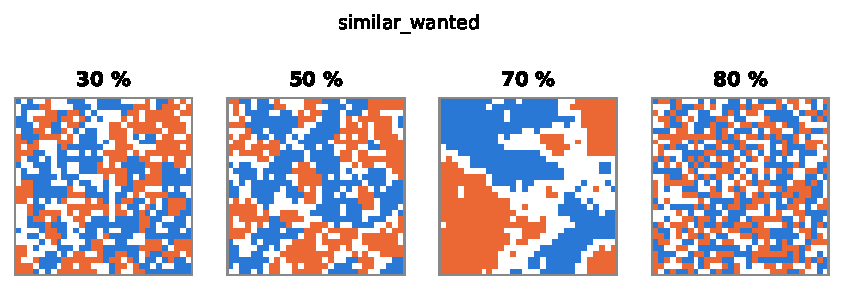
\includegraphics[width=\linewidth]{schelling_cartes.pdf}
  \caption{État final de la ville (\texttt{density} = 0.7, \texttt{distance} = 1) pour
  plusieurs valeurs de \texttt{similar\_wanted}. Les deux couleurs représentent les deux
  populations, le blanc les maisons vides. À 80\,\% la simulation ne converge pas.}
  \label{fig:schelling-cartes}
\end{figure}

\subsection{Pourcentage de similarité à l'équilibre}

Pour reproduire le transparent 23 du cours 2, nous avons ajouté au modèle la variable
\texttt{percent\_similar} : le nombre total de voisins de même couleur divisé par le nombre
total de voisins (définition de NetLogo), affichée dans un moniteur et sur le graphique
d'évolution. Une expérience \texttt{batch} fait ensuite varier \texttt{similar\_wanted}
de 10 à 90\,\% (\texttt{density} = 0.5, \texttt{distance} = 3, 5 répétitions par valeur,
arrêt à la convergence ou après 200 cycles).

\begin{table}[H]
  \centering
  \begin{tabular}{l*{9}{c}}
    \toprule
    \texttt{similar\_wanted} (\%) & 10 & 20 & 30 & 40 & 50 & 60 & 70 & 80 & 90 \\
    \midrule
    similarité à l'équilibre (\%) & 50,0 & 50,2 & 56,0 & 83,4 & 88,9 & 97,0 & 99,4 & 49,6 & 50,0 \\
    \bottomrule
  \end{tabular}
  \caption{Similarité moyenne à l'équilibre en fonction du seuil voulu (moyenne de 5 simulations).}
  \label{tab:schelling}
\end{table}

\begin{figure}[H]
  \centering
  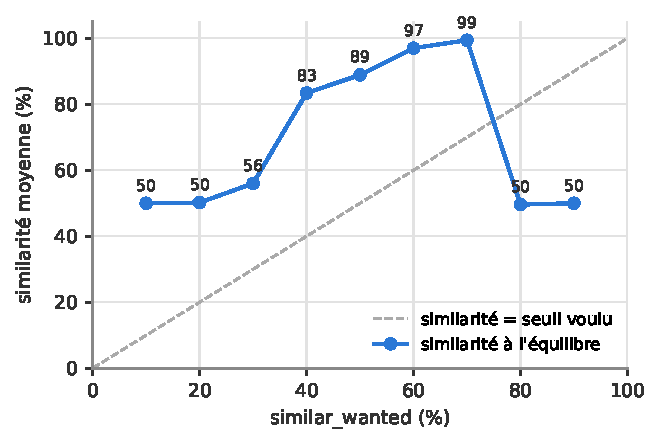
\includegraphics[width=0.62\linewidth]{schelling_similarite.pdf}
  \caption{Similarité à l'équilibre en fonction de \texttt{similar\_wanted}. La diagonale
  représente une similarité égale au seuil demandé.}
  \label{fig:schelling-sim}
\end{figure}

\paragraph{Analyse.}
\begin{itemize}
  \item Tant que le système converge, la similarité obtenue est \textbf{toujours supérieure}
  au seuil demandé : des
  préférences individuelles modérées (40\,\% de voisins semblables) produisent une
  ségrégation globale forte (83\,\%). C'est le résultat central de Schelling : le phénomène
  collectif n'est pas la simple somme des intentions individuelles.
  \item Le passage est \textbf{brutal entre 30 et 40\,\%}. En dessous, presque tous les agents
  sont déjà satisfaits par la configuration aléatoire initiale (environ 50\,\% de voisins
  semblables), il n'y a quasiment pas de déménagements. Au-dessus, chaque déménagement
  rend d'autres agents mécontents et une réaction en chaîne crée des zones homogènes.
  \item À partir de \textbf{80\,\%}, la similarité retombe à 50\,\% : le système ne
  converge plus, les agents ne trouvent jamais de place qui les satisfait et continuent de
  déménager au hasard, ce qui mélange la population.
\end{itemize}

%=====================================================================
\section{Dynamique d'opinions : le modèle \textit{Bounded Confidence}}
%=====================================================================

\subsection{Le modèle de base (question 2.1)}

Nous implémentons le modèle de la section 2.1 de Deffuant et al.\ (2001) dans
\texttt{BC\_Base.gaml}. Chaque agent possède une opinion $x \in [0,1]$, tirée uniformément
à l'initialisation. Deux agents d'opinions $x$ et $x'$ qui se rencontrent ne discutent que si
$|x - x'| < d$ (seuil de confiance). Ils se rapprochent alors selon
\begin{equation*}
  x \leftarrow x + \mu\,(x' - x), \qquad x' \leftarrow x' + \mu\,(x - x'),
\end{equation*}
où $\mu \in\, ]0, 0.5]$ est le paramètre de convergence.

\begin{lstlisting}[language=Java]
reflex discute when: not gel {
    SimpleAgent neighbor <- one_of(SimpleAgent);
    if (neighbor != self) {
        if (abs(neighbor.opinion - opinion) < threshold) {
            float temp <- opinion;
            opinion <- opinion + convergenceParam * (neighbor.opinion - opinion);
            neighbor.opinion <- neighbor.opinion
                                + convergenceParam * (temp - neighbor.opinion);
        }
    }
}
\end{lstlisting}

À chaque cycle, chaque agent choisit un partenaire au hasard dans toute la population :
un cycle correspond donc à $N$ rencontres, soit l'unité de temps de l'article
(1\,000 paires pour $N = 1\,000$).

\paragraph{Détection des pics.} Pour compter les groupes d'opinion, on trie les opinions et
on coupe dès que deux opinions consécutives sont à une distance $\ge d$. Deux groupes ainsi
séparés ne peuvent plus jamais interagir. Si de plus chaque groupe a une largeur $< d$,
tous ses membres peuvent encore discuter entre eux et le groupe ne fait que se resserrer :
la structure est alors \emph{définitive}. On appelle \emph{pic} un groupe contenant plus de
1\,\% des agents, ce qui exclut, comme dans l'article, les agents isolés et les « ailes »
proches de 0 ou 1. Ce critère sert aussi de condition d'arrêt exacte pour les expériences
\texttt{batch}.

\subsection{Premiers essais avec 50 agents (question 2.2)}

\begin{itemize}
  \item Les opinions se regroupent en quelques dizaines de cycles, puis plus rien ne change :
  chaque groupe s'est contracté sur une valeur unique et les groupes sont à plus de $d$ les
  uns des autres. Prolonger la simulation ne modifie rien.
  \item Avec $d = 0.3$, on obtient en général un seul groupe autour de 0.5 (parfois deux),
  plus quelques agents isolés près de 0 ou de 1. Avec $d = 0.1$, on obtient 4 à 5 groupes.
  \item Un $\mu$ plus faible donne le même résultat final, mais plus lentement.
  \item Avec seulement 50 agents, le résultat varie beaucoup d'une simulation à l'autre
  (effet de taille finie), et les agents isolés pèsent relativement plus.
\end{itemize}

\subsection{Reproduction des figures 1 et 2 (question 2.3.1)}

\begin{figure}[H]
  \centering
  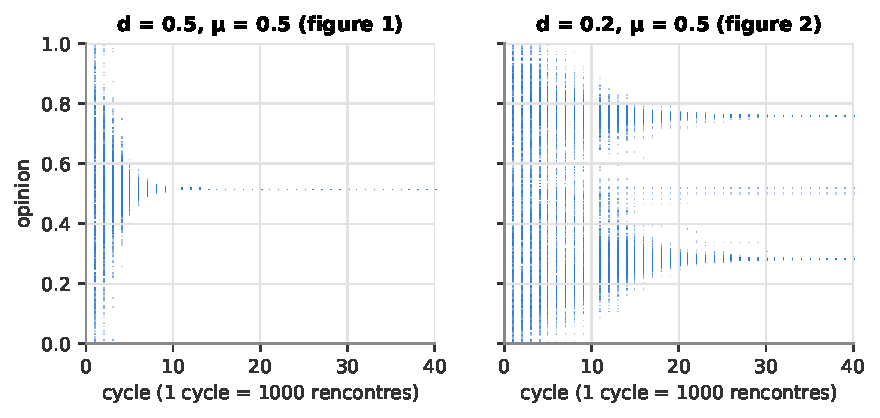
\includegraphics[width=\linewidth]{bc_trajectoires.pdf}
  \caption{Évolution des opinions de 1\,000 agents (expérience \texttt{BC\_Base\_1000}).
  À gauche, consensus ; à droite, deux pics principaux, plus ici un petit groupe isolé
  vers 0.5 qui contient trop peu d'agents pour compter comme un pic.}
  \label{fig:trajectoires}
\end{figure}

\begin{itemize}
  \item \textbf{Figure 1} ($d = 0.5$, $\mu = 0.5$) : on obtient bien un \textbf{consensus}
  autour de 0.5, la moyenne des opinions initiales. La structure est fixée en environ 5 cycles
  et toutes les opinions sont confondues après 20 à 30 cycles.
  \item \textbf{Figure 2} ($d = 0.2$, $\mu = 0.5$) : on obtient bien \textbf{deux pics},
  vers 0.25--0.3 et 0.7--0.75 (l'article : $\approx 0.25$ et $\approx 0.73$), avec parfois
  un ou deux agents isolés entre les deux, comme le point vers 0.55 de la figure 2.
\end{itemize}
Les figures sont donc reproduites qualitativement. Si l'axe des abscisses de l'article
compte des rencontres individuelles, nos 20 à 30 cycles de 1\,000 rencontres sont du même
ordre de grandeur que la convergence visible sur la figure 1.

\begin{figure}[H]
  \centering
  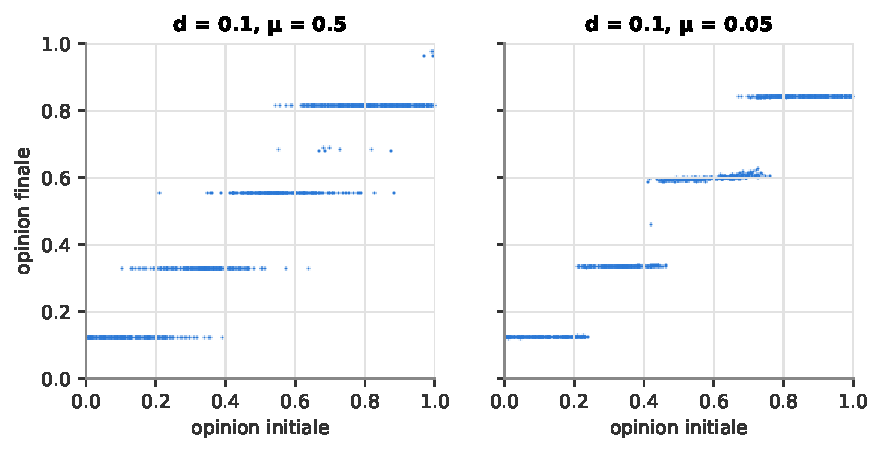
\includegraphics[width=\linewidth]{bc_figure3.pdf}
  \caption{Opinion finale en fonction de l'opinion initiale ($d = 0.1$), équivalent de la
  figure 3 de l'article. Avec $\mu = 0.05$ les marches sont plus nettes : les agents
  rejoignent presque toujours le pic le plus proche.}
  \label{fig:figure3}
\end{figure}

\subsection{Effet des paramètres (question 2.3.2)}

L'expérience \texttt{Effet\_parametres} fait varier $d$, $\mu$ et $N$ (5 simulations par
combinaison) et mesure le nombre de pics et le nombre de cycles avant que la structure soit
définitive.

\begin{table}[H]
  \centering
  \begin{tabular}{lcccc}
    \toprule
    $d$ \textbackslash{} $\mu$ & 0.05 & 0.1 & 0.3 & 0.5 \\
    \midrule
    0.1 & 343 (4.2) & 203 (4.0) & 70 (4.2) & 59 (4.8) \\
    0.2 & 150 (2.0) & 72 (2.0) & 32 (2.0) & 28 (2.0) \\
    0.3 & 65 (1.0) & 35 (1.0) & 17 (1.0) & 14 (1.0) \\
    0.5 & 20 (1.0) & 10 (1.0) & 6 (1.0) & 5 (1.0) \\
    \bottomrule
  \end{tabular}
  \caption{Nombre de cycles avant structure définitive pour $N = 1\,000$ (nombre moyen de
  pics entre parenthèses).}
  \label{tab:effet}
\end{table}

\begin{figure}[H]
  \centering
  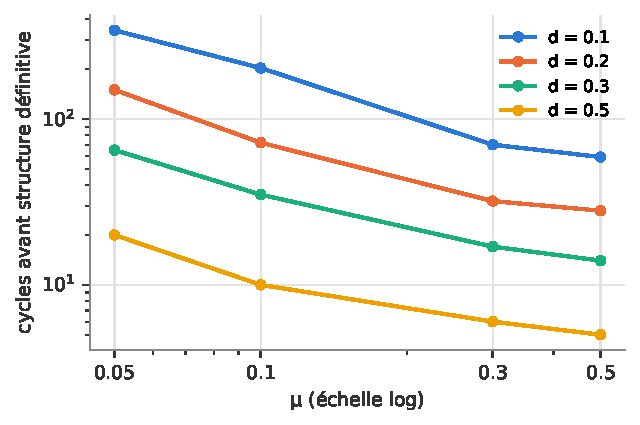
\includegraphics[width=0.6\linewidth]{bc_convergence.pdf}
  \caption{Temps de convergence en fonction de $\mu$ pour différentes valeurs de $d$
  ($N = 1\,000$, échelles logarithmiques).}
  \label{fig:convergence}
\end{figure}

\begin{itemize}
  \item \textbf{$d$} décide du résultat : un grand $d$ mène au consensus, un petit $d$ à
  plusieurs pics (environ $1/(2d)$, voir section suivante). Avec un petit $d$, chaque agent
  n'écoute que ceux qui pensent déjà comme lui : des groupes se forment puis deviennent étanches.
  \item \textbf{$\mu$} ne change pas le nombre de pics, seulement la \textbf{vitesse} :
  le temps de convergence est à peu près proportionnel à $1/\mu$ (343 cycles pour
  $\mu = 0.05$ contre 59 pour $\mu = 0.5$ à $d = 0.1$). Un grand $\mu$ laisse un peu plus
  d'agents hors des pics : le nombre total de groupes, isolés compris, passe de 4.6 à 6.4
  à $d = 0.1$ quand $\mu$ passe de 0.05 à 0.5. Avec un petit $\mu$, les agents « ont le temps
  de se décider » et rejoignent le pic le plus proche (figure~\ref{fig:figure3}).
  \item \textbf{$N$} ne change pas qualitativement la structure (1 pic pour $d \ge 0.3$,
  2 pour $d = 0.2$, avec $N = 100$ comme avec $N = 1\,000$), mais les fluctuations d'une
  simulation à l'autre sont plus fortes pour les petites populations.
  \item Plus $d$ est petit, plus la convergence est lente : chaque agent trouve moins souvent
  un partenaire assez proche pour discuter.
\end{itemize}

\subsection{Nombre de pics en fonction de $d$ : la figure 4 (question 2.4)}

L'expérience \texttt{Figure4} lance, pour 28 valeurs de $d$ entre 0.05 et 0.5, des
simulations à $N = 1\,000$ et $\mu = 0.5$ arrêtées dès que la structure est définitive, et
compte le nombre de pics. Les résultats agrègent 7 lancements, soit 70 simulations par valeur
de $d$ (l'article en utilise 250).

\begin{figure}[H]
  \centering
  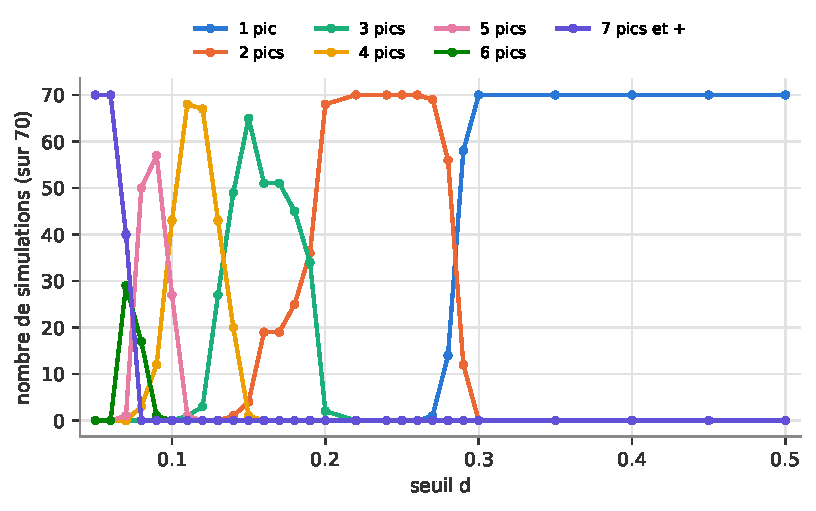
\includegraphics[width=0.9\linewidth]{bc_figure4.pdf}
  \caption{Nombre de simulations (sur 70) se terminant avec $k$ pics, en fonction de $d$.
  Équivalent de la figure 4 de l'article.}
  \label{fig:figure4}
\end{figure}

\begin{table}[H]
  \centering
  \small
  \begin{tabular}{lccccccccc}
    \toprule
    $d$ & 1 & 2 & 3 & 4 & 5 & 6 & 7+ & moyenne & $1/(2d)$ \\
    \midrule
    0.05 & 0 & 0 & 0 & 0 & 0 & 0 & 70 & 8.20 & 10.00 \\
    0.07 & 0 & 0 & 0 & 0 & 1 & 29 & 40 & 6.56 & 7.14 \\
    0.08 & 0 & 0 & 0 & 3 & 50 & 17 & 0 & 5.20 & 6.25 \\
    0.10 & 0 & 0 & 0 & 43 & 27 & 0 & 0 & 4.39 & 5.00 \\
    0.12 & 0 & 0 & 3 & 67 & 0 & 0 & 0 & 3.96 & 4.17 \\
    0.13 & 0 & 0 & 27 & 43 & 0 & 0 & 0 & 3.61 & 3.85 \\
    0.15 & 0 & 4 & 65 & 1 & 0 & 0 & 0 & 2.96 & 3.33 \\
    0.19 & 0 & 36 & 34 & 0 & 0 & 0 & 0 & 2.49 & 2.63 \\
    0.20 & 0 & 68 & 2 & 0 & 0 & 0 & 0 & 2.03 & 2.50 \\
    0.25 & 0 & 70 & 0 & 0 & 0 & 0 & 0 & 2.00 & 2.00 \\
    0.28 & 14 & 56 & 0 & 0 & 0 & 0 & 0 & 1.80 & 1.79 \\
    0.29 & 58 & 12 & 0 & 0 & 0 & 0 & 0 & 1.17 & 1.72 \\
    0.30 & 70 & 0 & 0 & 0 & 0 & 0 & 0 & 1.00 & 1.67 \\
    \bottomrule
  \end{tabular}
  \caption{Extrait des résultats : nombre de simulations ayant $k$ pics (tableau complet dans
  \texttt{resultats/figure4\_agrege.csv}).}
  \label{tab:figure4}
\end{table}

\paragraph{Comparaison avec l'article.} On retrouve la figure 4 : une succession de
\textbf{plateaux} où toutes les simulations ont le même nombre de pics, séparés par des
\textbf{transitions étroites} où deux nombres de pics coexistent. La transition de 2 à 1 pic
a lieu vers $d \approx 0.28$ (article : $\approx 0.27$), celle de 3 à 2 pics vers
$d \approx 0.19$ (article : $\approx 0.19$), puis 4$\to$3 vers 0.13, 5$\to$4 vers 0.10,
6$\to$5 vers 0.08 et 7$\to$6 vers 0.07.

\begin{figure}[H]
  \centering
  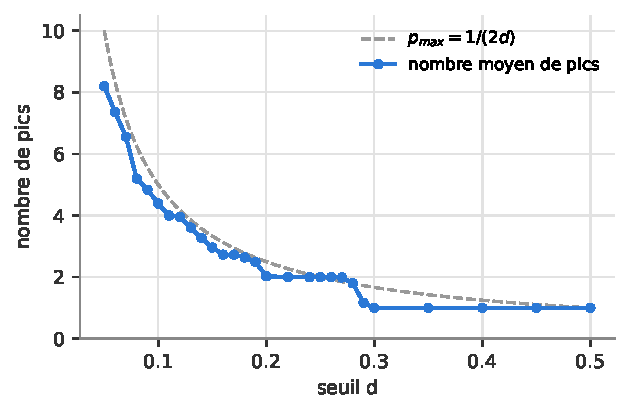
\includegraphics[width=0.6\linewidth]{bc_moyenne_pics.pdf}
  \caption{Nombre moyen de pics comparé à la borne $p_{max} = 1/(2d)$ de l'article.}
  \label{fig:moyenne}
\end{figure}

\paragraph{Explication.} Un agent n'est influencé que par les opinions situées à moins de $d$
de la sienne : il se rapproche de la moyenne de l'intervalle $[x - d, x + d]$. Les zones un
peu plus denses attirent donc leurs voisines, les « vallées » se vident et les opinions se
concentrent en pics (c'est le sens de l'équation de diffusion donnée dans l'article). Deux pics
ne survivent côte à côte que s'ils sont à plus de $d$ l'un de l'autre ; comme les opinions
intermédiaires sont absorbées, les pics finaux sont espacés d'environ $2d$. Les agents
proches des bords 0 et 1 n'ont de voisins que d'un côté et dérivent vers l'intérieur d'environ
$d$. On peut donc placer au plus environ $1/(2d)$ pics dans $[0, 1]$, ce qui donne la borne
$p_{max}$ de l'article. Le nombre moyen observé reste \textbf{un peu en dessous} de cette
borne (figure~\ref{fig:moyenne}), et dans les zones de transition c'est le tirage aléatoire des
opinions initiales qui décide s'il reste un pic de plus ou de moins.

%---------------------------------------------------------------------
\subsection{Effet des réseaux sociaux : modèle sur grille (question 2.5)}
%---------------------------------------------------------------------

Le fichier \texttt{BC\_Grid.gaml} adapte le modèle à un voisinage social, comme dans la
section 3 de l'article.
\begin{itemize}
  \item La population est une \textbf{grille 29$\times$29} (841 agents) dont chaque cellule
  est un agent portant une opinion ; toutes les cases étant occupées, une espèce séparée
  n'est pas nécessaire.
  \item \texttt{neighbors: 4} donne le \textbf{voisinage de Von Neumann} (N, S, E, O), sans
  tore. Remplacer par \texttt{neighbors: 8} donne le voisinage de Moore.
  \item À chaque cycle, chaque cellule choisit un de ses voisins au hasard (attribut
  \texttt{neighbors} de la grille) et applique la règle BC. Un cycle fait 841 rencontres ;
  les 100\,000 itérations de l'article correspondent à environ 120 cycles.
  \item Affichage : grille en niveaux de gris (0 = noir, 1 = blanc) comme les figures 5 et 6,
  plus grand cluster en rouge, et histogramme à 101 classes comme la figure 7.
  \item Analyse : on calcule les \textbf{clusters spatiaux}, composantes connexes de la grille
  où deux voisins sont reliés si $|x - x'| < d$ (parcours en largeur). On mesure leur nombre,
  le nombre d'agents isolés (aucun voisin à moins de $d$ : ils ne bougeront plus jamais),
  la taille du plus grand cluster et s'il \emph{percole}, c'est-à-dire s'il relie deux bords
  opposés de la grille.
  \item Paramètres : \texttt{threshold} ($d$), \texttt{convergenceParam} ($\mu$),
  \texttt{stop\_cycle} et \texttt{grid\_size}.
\end{itemize}

\subsection{Comparaison avec les figures 5, 6 et 7 (question 2.6)}

\begin{figure}[H]
  \centering
  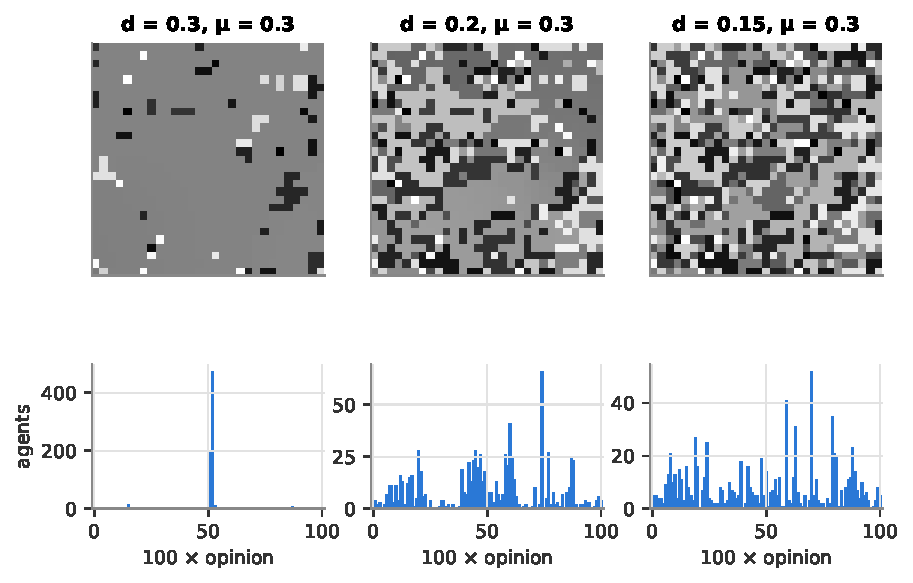
\includegraphics[width=0.95\linewidth]{grid_cartes.pdf}
  \caption{Opinions finales sur la grille après 1\,000 cycles ($\mu = 0.3$) et histogrammes
  correspondants (101 classes, comme la figure 7).}
  \label{fig:grilles}
\end{figure}

\begin{table}[H]
  \centering
  \begin{tabular}{cccccc}
    \toprule
    $d$ & clusters & clusters $> 1\,\%$ & agents isolés & plus grand cluster & percolation \\
    \midrule
    0.10 & 505 & 5.6 & 357 (42\,\%) & 1.8\,\% & 0\,\% \\
    0.15 & 333 & 15.8 & 204 (24\,\%) & 5.4\,\% & 0\,\% \\
    0.20 & 182 & 9.4 & 109 (13\,\%) & 35.7\,\% & 80\,\% \\
    0.25 & 90 & 6.6 & 48 (6\,\%) & 71.6\,\% & 100\,\% \\
    0.30 & 37 & 1.0 & 25 (3\,\%) & 92.9\,\% & 100\,\% \\
    0.40 & 14 & 1.0 & 11 (1\,\%) & 98.1\,\% & 100\,\% \\
    0.50 & 1 & 1.0 & 0 & 100\,\% & 100\,\% \\
    \bottomrule
  \end{tabular}
  \caption{Statistiques des clusters à l'équilibre ($\mu = 0.3$, moyenne de 5 simulations,
  expérience \texttt{Grid\_Stats}). La colonne percolation donne la proportion de simulations
  où le plus grand cluster relie deux bords opposés.}
  \label{tab:grille}
\end{table}

\begin{figure}[H]
  \centering
  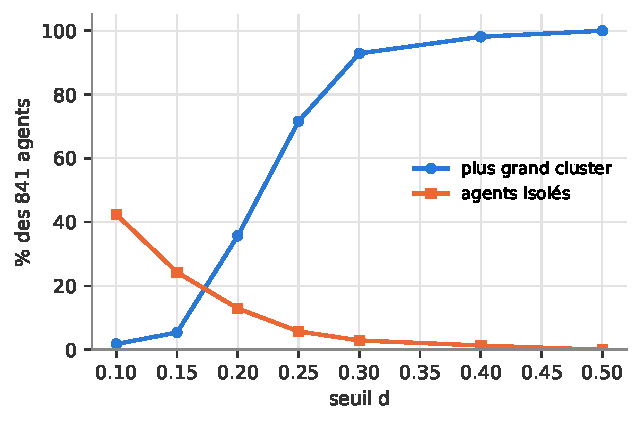
\includegraphics[width=0.6\linewidth]{grid_stats.pdf}
  \caption{Taille du plus grand cluster et proportion d'agents isolés en fonction de $d$
  ($\mu = 0.3$).}
  \label{fig:grid-stats}
\end{figure}

\paragraph{Figure 5 ($d = 0.3$, $\mu = 0.3$) : reproduite.} Un grand cluster d'opinion
homogène autour de 0.5 occupe environ 93\,\% de la grille et percole ; il reste une
vingtaine d'agents isolés aux opinions proches de 0 ou 1, les « extrémistes » de l'article.

\paragraph{Figure 6 ($d = 0.15$, $\mu = 0.3$) : partiellement reproduite.} On observe bien
la fragmentation en nombreux clusters non percolants d'opinions « semblables mais pas
égales ». En revanche, nous n'obtenons \textbf{pas le grand cluster percolant} de l'article :
le plus grand cluster ne contient qu'environ 5\,\% des agents, et un quart des agents restent
isolés. Une réimplémentation indépendante (en Python, avec ou sans tore) donne le même
résultat. Avec le modèle tel qu'il est décrit, la percolation n'apparaît qu'à partir de
$d \approx 0.2$ et devient systématique à $d = 0.25$. Cela s'explique simplement : au départ,
un agent a une probabilité d'environ $(1 - 2d + d^2)^4 \approx 0.27$ de n'avoir \emph{aucun}
de ses 4 voisins à moins de $d = 0.15$. Il est alors gelé définitivement et coupe le réseau.
L'article a probablement utilisé une variante (procédure de rencontre, initialisation ou
valeur de $d$) qu'il ne précise pas.

\paragraph{Figure 7.} Pour $d = 0.15$, l'histogramme est beaucoup plus étalé que les pics
très fins du modèle de base : chaque cluster non connecté converge vers sa propre moyenne
locale.

\paragraph{Effets du voisinage social.}
\begin{enumerate}
  \item Pour $d \ge 0.3$, le résultat ressemble à celui du modèle de base (consensus), mais
  avec \textbf{beaucoup plus d'agents isolés}. En mélange complet, un agent marginal finit
  toujours par rencontrer quelqu'un d'assez proche ; sur la grille, il ne parle qu'à ses
  4 voisins et, si aucun n'est assez proche, il reste bloqué.
  \item Pour $d$ petit, le nombre de groupes \textbf{n'est plus du tout $1/(2d)$} : au lieu
  de 3 pics à $d = 0.15$ on obtient des centaines de clusters. Le consensus ne peut se faire
  qu'entre agents connectés : deux clusters d'opinions presque égales qui ne se touchent pas
  ne fusionnent jamais.
  \item La structure finale dépend de la géométrie locale et de l'histoire de chaque région,
  d'où une plus grande variabilité d'une simulation à l'autre, comme le note l'article.
  \item La convergence est \textbf{beaucoup plus lente} (des centaines à des milliers de
  cycles au lieu de quelques dizaines) : l'influence se propage de proche en proche.
\end{enumerate}

\paragraph{Effet des paramètres.} Comme pour le modèle de base, $\mu$ ne change que la
vitesse (à $d = 0.1$ : 832, 286 et 180 cycles pour $\mu = 0.1$, $0.3$ et $0.5$) et non la
structure : le nombre de clusters, la taille du plus grand cluster et le nombre d'isolés sont
quasiment identiques pour les trois valeurs. Le seuil $d$ reste le paramètre clé, mais son
effet n'est plus « nombre de pics $\approx 1/(2d)$ » : on observe une \textbf{transition de
percolation}. En dessous de $d \approx 0.2$ la population est fragmentée ; au-dessus, un
cluster géant englobe rapidement presque tout le monde (figure~\ref{fig:grid-stats}).

%---------------------------------------------------------------------
\subsection{Extension : influence des extrémistes}
%---------------------------------------------------------------------

\paragraph{Implémentation (question 2.6.1).} Le fichier \texttt{BC\_Grid\_Extremistes.gaml}
part du modèle sur grille. Les opinions sont dans $[-1, 1]$ comme dans l'énoncé, ce qui double
toutes les distances : $d = 0.6$ ici correspond à $d = 0.3$ sur $[0, 1]$. $NE$ cellules tirées
au hasard sont extrémistes : leur opinion vaut $+1$ (ou $\pm 1$ avec deux camps) et n'est
jamais modifiée, mais elles influencent un voisin suffisamment proche avec la même règle.
On mesure le pourcentage d'agents normaux \emph{capturés} (opinion $> 0.8$) et leur opinion
moyenne ; $NE = 0$ sert de référence, car même sans extrémistes quelques agents isolés restent
près de $\pm 1$.

\begin{figure}[H]
  \centering
  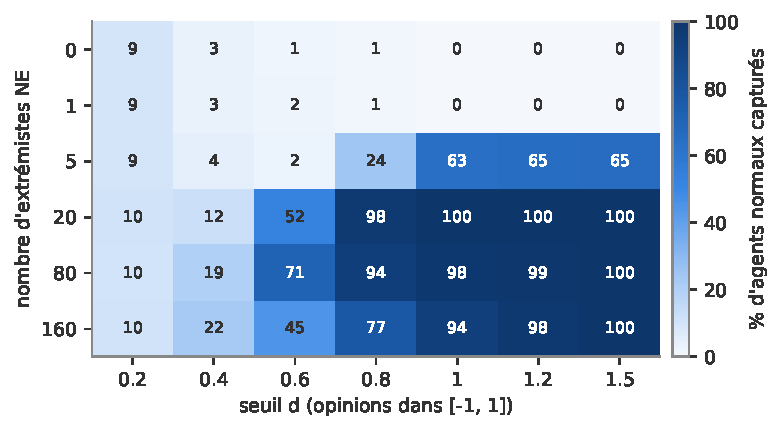
\includegraphics[width=0.72\linewidth]{extremistes_tableau.pdf}
  \caption{Pourcentage d'agents normaux capturés par les extrémistes ($+1$), en fonction du
  nombre d'extrémistes et du seuil $d$ (opinions dans $[-1, 1]$, $\mu = 0.3$, 5 simulations
  par case, 1\,000 cycles au maximum).}
  \label{fig:extremistes}
\end{figure}

\begin{figure}[H]
  \centering
  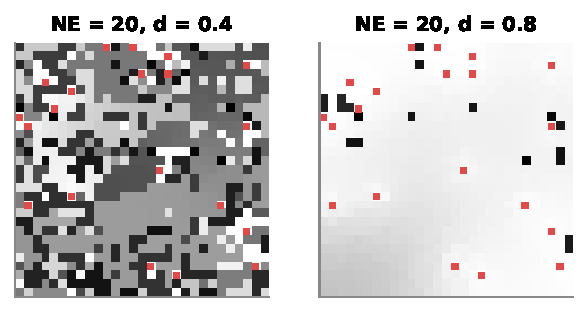
\includegraphics[width=0.6\linewidth]{extremistes_grilles.pdf}
  \caption{État de la grille après 500 cycles avec 20 extrémistes (carrés rouges).
  Avec $d = 0.4$ leur influence reste locale ; avec $d = 0.8$ presque toute la population
  est attirée vers $+1$ (blanc).}
  \label{fig:extremistes-grilles}
\end{figure}

\paragraph{Combien d'extrémistes faut-il ?} La réponse dépend surtout de $d$ :
\begin{itemize}
  \item \textbf{$d \le 0.4$} ($\le 0.2$ sur $[0,1]$) : les extrémistes ne capturent que leur
  voisinage immédiat, quel que soit leur nombre. Même avec 160 extrémistes (19\,\% de la
  population), seuls 20\,\% environ des agents normaux sont capturés et l'opinion moyenne
  ne bouge pas.
  \item \textbf{$d = 0.6$} ($0.3$ sur $[0,1]$) : il faut une vingtaine d'extrémistes (2 à 3\,\%
  de la population) pour capturer la moitié des agents.
  \item \textbf{$d \ge 0.8$} : quelques extrémistes suffisent. 5 extrémistes (0.6\,\%)
  capturent 25 à 65\,\% des agents, et 20 (2.4\,\%) en capturent presque 100\,\%.
  \item \textbf{$d \ge 1$} : même un seul extrémiste déplace toute la population, car le
  consensus central reste à moins de $d$ de $+1$ et est tiré en permanence. Après 1\,000
  cycles l'opinion moyenne est déjà à 0.24 et continue d'augmenter.
\end{itemize}

\paragraph{Lien avec les autres paramètres (question 2.6.2).} Il s'agit d'une course entre
deux processus : la population modérée converge vers le centre, tandis que les extrémistes
tirent leurs voisins vers $+1$. Dès que le consensus central est formé à une distance $\ge d$
des extrémistes, ceux-ci sont isolés et n'ont plus aucun effet. Leur influence passe donc par
des \emph{chaînes d'agents relais} distants de moins de $d$ ; plus $d$ est grand, plus ces
chaînes existent et plus le consensus lui-même reste à leur portée. On retrouve le résultat
de Deffuant et al.\ (2002) : les extrémistes l'emportent quand l'incertitude des modérés est
grande. On observe aussi un effet non monotone de $NE$ à $d = 0.6$ et $0.8$ : 160 extrémistes
capturent moins que 80. Sur une grille, des extrémistes nombreux occupent des cases et coupent
le réseau des modérés, ce qui raccourcit les chaînes de relais. Ce point est à confirmer
avec plus de répétitions. Enfin, $\mu$ devrait surtout jouer sur la vitesse ; un grand $\mu$
peut toutefois former le consensus central plus vite et isoler les extrémistes plus tôt.

%---------------------------------------------------------------------
\subsection{Limites du modèle et améliorations (question 2.7)}
%---------------------------------------------------------------------

\paragraph{Limites.}
\begin{itemize}
  \item L'opinion est réduite à un nombre, alors qu'une attitude a une composante cognitive,
  affective, sociale et comportementale.
  \item Tous les agents ont le même seuil $d$ et la même influence $\mu$, et l'influence est
  symétrique. En réalité, l'ouverture d'esprit et la crédibilité varient d'un individu à
  l'autre ; les extrémistes sont en général plus sûrs d'eux.
  \item Il n'y a pas d'influence négative (rejet) : les agents ne peuvent que se rapprocher,
  le modèle ne peut donc pas expliquer une polarisation croissante.
  \item Il n'y a ni bruit ni information extérieure (médias, expérience personnelle) : les
  états finaux sont figés pour toujours.
  \item Le réseau est soit complet, soit une grille régulière et statique, alors que les
  réseaux sociaux réels sont de type « petit monde », avec des individus très connectés,
  et évoluent avec les opinions.
  \item L'échelle de temps est arbitraire et les paramètres ne sont pas calibrés sur des
  données.
\end{itemize}

\paragraph{Améliorations prioritaires.}
\begin{enumerate}
  \item Des seuils hétérogènes et évolutifs, comme dans le modèle \textit{Relative Agreement}
  (Deffuant et al., 2002), où chaque agent a sa propre incertitude.
  \item Des réseaux sociaux plus réalistes (petit monde, sans échelle), éventuellement
  dynamiques.
  \item Du bruit, des sources extérieures et de l'influence négative.
  \item Des opinions multidimensionnelles, puis des modèles plus cognitifs fondés sur les
  attitudes et les normes sociales, calibrés sur des données.
\end{enumerate}

%=====================================================================
\section*{Conclusion}
\addcontentsline{toc}{section}{Conclusion}
%=====================================================================

Les deux modèles étudiés montrent comment des règles locales très simples produisent des
structures collectives que les agents n'ont pas cherchées : une ségrégation forte à partir
de préférences modérées chez Schelling, et des groupes d'opinion étanches dans le modèle
\textit{Bounded Confidence}. Dans ce dernier, le seuil de confiance $d$ détermine presque à
lui seul le résultat : nombre de pics en $1/(2d)$ en mélange complet, transition de percolation
sur une grille, et capacité de quelques extrémistes à faire basculer une population. Ces
modèles restent cependant très simplifiés, et des modèles plus descriptifs et cognitifs sont
nécessaires pour étudier des situations réelles.


\end{document}
